\begin{task}
\TT{Oblicz wartość skuteczną okresowego sygnału $f(t)$ przedstawionego na rysunku:}{Calculate the effective (RMS) value of the following periodic signal $f(t)$:}

\begin{figure}[H]
\centering
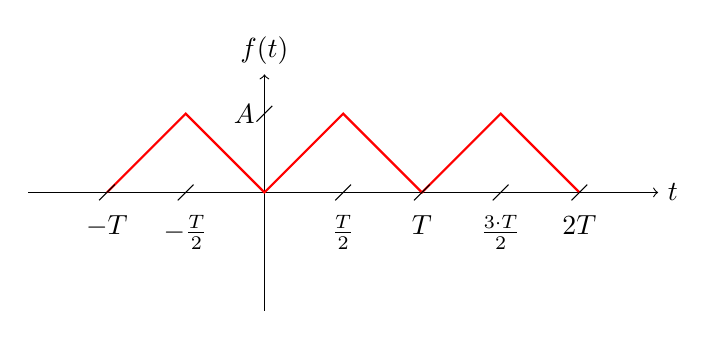
\begin{tikzpicture}
  %\draw (0,0) circle (1in);
  \draw[->] (-3.0,+0.0) -- (+5.0,+0.0) node[right] {$t$};
  \draw[->] (+0.0,-1.5) -- (+0.0,+1.5) node[above] {$f(t)$};
  \draw[-,red, thick] (-2.0,+0.0) -- (-1.0,+1.0) --(+0.0,+0.0) -- (+1.0,+1.0) -- (+2.0,+0.0) -- (3.0,1.0) -- (4.0,0.0);
  \draw[-] (-2.0-0.1,-0.1)--(-2.0+0.1,0.1) node[midway, below, outer sep=5pt,align=center] {$-T$};
  \draw[-] (-1.0-0.1,-0.1)--(-1.0+0.1,0.1) node[midway, below, outer sep=5pt,align=center] {$-\frac{T}{2}$};
  \draw[-] (+1.0-0.1,-0.1)--(+1.0+0.1,0.1) node[midway, below, outer sep=5pt] {$\frac{T}{2}$};
  \draw[-] (+2.0-0.1,-0.1)--(+2.0+0.1,0.1) node[midway, below, outer sep=5pt] {$T$};
  \draw[-] (+3.0-0.1,-0.1)--(+3.0+0.1,0.1) node[midway, below, outer sep=5pt] {$\frac{3 \cdot T}{2}$};
  \draw[-] (+4.0-0.1,-0.1)--(+4.0+0.1,0.1) node[midway, below, outer sep=5pt] {$2T$};
  \draw[-] (-0.1,1.0-0.1)--(+0.1,1.0+0.1) node[midway, left] {$A$};
\end{tikzpicture}
\end{figure}

\TT{Zaczynamy od zapisania wzoru funkcji przedstawionej na rysunku:}{Signal $f(t)$ can de described as:}

\begin{equation}
   f(x)=\begin{cases}\frac{2 \cdot A}{T} \cdot (t - k \cdot T) & t \in \left (  0+k \cdot T; \frac{T}{2}+k \cdot T \right ) \\
   -\frac{2 \cdot A}{T} \cdot (t - k \cdot T) & t \in \left ( -\frac{T}{2}+k \cdot T; 0 +k \cdot T\right )\end{cases} \wedge k \in \TT{C}{Z}
\end{equation}

\TT{Wartość skuteczną sygnału okresowego wyznaczamy ze wzoru:}{The effective (RMS) value for periodic signals is defined by:}

\begin{equation}
\begin{aligned}
\TT{U_{sk}}{U_{RMS}}&=\sqrt{P}\\
P=&\frac{1}{T} \cdot \int_{T}^{}\left|f(t)\right|^2 \cdot dt
\end{aligned}
\end{equation}

\TT{Podstawiamy do wzoru na moc wzór naszej funkcji dla pierwszego okresu $k=0$}{Compute average power for period $k=0$}

\begin{align*}
	P&=\frac{1}{T} \cdot \int_{T}\left|f(t)\right|^2 \cdot dt =\\
	&=\frac{1}{T} \cdot \left( \int_{-\frac{T}{2}}^{0}\left| \left(-\frac{2 \cdot A}{T} \cdot t \right) \right|^2 \cdot dt + \int_{0}^{\frac{T}{2}}\left| \left(\frac{2 \cdot A}{T} \cdot t \right) \right|^2 \cdot dt\right)=\\
	&=\frac{1}{T} \cdot \left( \int_{-\frac{T}{2}}^{0} \left(-\frac{2 \cdot A}{T} \cdot t \right)^2 \cdot dt + \int_{0}^{\frac{T}{2}}\left(\frac{2 \cdot A}{T} \cdot t \right)^2 \cdot dt\right)=\\
	&=\frac{1}{T} \cdot \left( \int_{-\frac{T}{2}}^{0}\frac{4 \cdot A^2}{T^2} \cdot t^2 \cdot dt + \int_{0}^{\frac{T}{2}} \frac{4 \cdot A^2}{T^2} \cdot t^2 \cdot dt\right)=\\
	&=\frac{4 \cdot A^2}{T^3} \cdot \left( \int_{-\frac{T}{2}}^{0} t^2 \cdot dt + \int_{0}^{\frac{T}{2}} t^2 \cdot dt\right)=\\
	&=\frac{4 \cdot A^2}{T^3} \cdot \left( \left. \frac{t^3}{3} \right|_{-\frac{T}{2}}^{0} +  \left. \frac{t^3}{3} \right|_{0}^{\frac{T}{2}} \right)=\\
	&=\frac{4 \cdot A^2}{3 \cdot T^3} \cdot \left( 0^3 - \left(-\frac{T}{2}\right)^3 + \left(\frac{T}{2}\right)^3 - 0^3 \right)=\\
	&=\frac{4 \cdot A^2}{3 \cdot T^3} \cdot \left( \frac{T^3}{8} + \frac{T^3}{8} \right)=\\
	&=\frac{4 \cdot A^2}{3 \cdot T^3} \cdot \left( \frac{T^3}{4} \right)=\\
	&=\frac{A^2}{3}\\
\end{align*}

\TT{Moc sygnału wynosi $\frac{A^2}{3}$.}{Average power equals to $\frac{A^2}{3}.$}

\begin{equation}
\begin{aligned}
\TT{U_{sk}}{U_{RMS}}&=\sqrt{P}\\
\TT{U_{sk}}{U_{RMS}}&=\sqrt{\frac{A^2}{3}}	\\
\TT{U_{sk}}{U_{RMS}}&=\frac{A}{\sqrt{3}}	
\end{aligned}
\end{equation}

\TT{Wartość skuteczna sygnału wynosi $\frac{A}{\sqrt{3}}$.}{Effective (RMS) value equals to $\frac{A}{\sqrt{3}}.$}

\end{task}